A probléma egy 1D doboba zárt résecske homogén erőtérben. $F(x)=-F$, azaz $V(x) = Fx$.
	Az egyenlethez tartozó határfeltételek, ha a doboz hossza $L$:
	\begin{equation}
		\psi \big\rvert_0 = \psi \big \rvert_L = 0
	\end{equation}
	A megoldandó időfüggetlen Schrödinger-egyenlet:
	\begin{equation}
		-\frac{\hbar^2}{2m}\frac{d^2\psi}{dx^2} + Fx\psi = E\psi
	\end{equation}
	\begin{equation}
		\frac{d^2\psi}{dx^2} - \frac{2mFx}{\hbar^2}\psi = -\frac{2mE}{\hbar^2}\psi
	\end{equation}
	\begin{equation}
		\frac{d^2\psi}{dx^2} - \left(\frac{2mF}{\hbar^2}x - \frac{2mE}{\hbar^2}\right)\psi = 0
	\end{equation}
	Az Airy egyenlet ilyen alakra hozható a változó affin lineáris transzformációjával:
	\begin{equation}
		\frac{d^2y}{dx^{\prime 2}} - x^\prime y = 0
	\end{equation}
	$x^\prime = ax - b$, azaz $\frac{d}{dx} = a\frac{d}{dx^\prime}$:
	\begin{equation}
		\frac{d^2y}{dx^2} - \left(a^3x - a^2b\right)y = 0
	\end{equation}
	Az együtthatók összevetése alapján $a = \sqrt[3]{\frac{2mF}{\hbar^2}}$ és $b = \sqrt[3]{\frac{2m}{\hbar^2F^2}}E$. Így a Schrödinger-gyenlet megoldása:
	\begin{equation}
		\psi(x) = y(x^\prime) = y\left(\sqrt[3]{\frac{2mF}{\hbar^2}}x - \sqrt[3]{\frac{2m}{\hbar^2F^2}}E\right)
	\end{equation}
	, ahol $y(x) = \alpha \Ai{x} + \beta \Bi{x}$.
	A $\psi \big\rvert_0 = 0$ feltételből következik, hogy $\psi \propto \Bi{-b}\Ai{ax-b} - \Ai{-b}\Bi{ax-b}$. A második határfeltétel pedig meghatározza a lehetséges energiákat. A feltétel:
	\begin{equation}
		\Bi{-b}\Ai{aL-b} - \Ai{-b}\Bi{aL-b} = 0
	\end{equation}
	\begin{equation}
		\label{box_energiaszintek_egyenlet}
		\Ti{aL-b} - \Ti{-b} = 0
	\end{equation}
	\begin{equation}
		\Ti{\sqrt[3]{\frac{2mF}{\hbar^2}}L - \sqrt[3]{\frac{2m}{\hbar^2F^2}}E} - \Ti{-\sqrt[3]{\frac{2m}{\hbar^2F^2}}E} = 0
	\end{equation}
	\begin{figure}[H]
		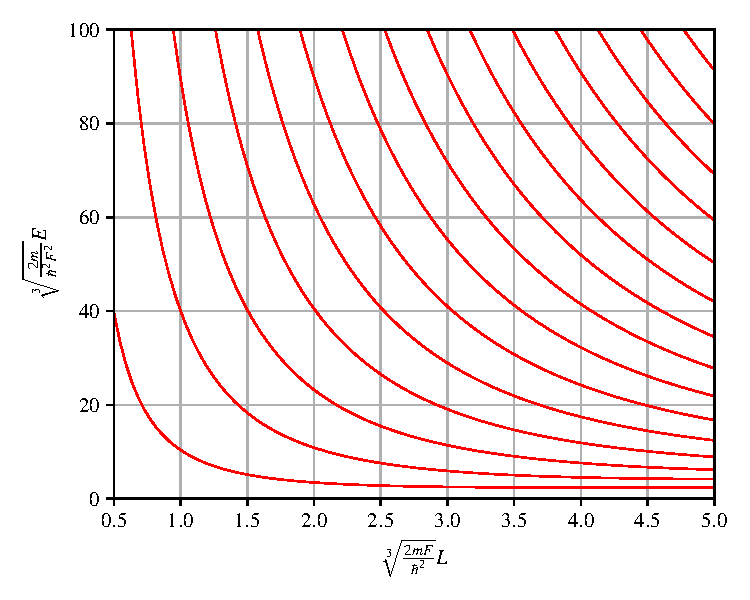
\includegraphics[scale=1]{./figs/energiaszintek.pdf}
		\caption{Energiaszintek $L$ függvényében}
		\label{box_energiaszintek_abra}
	\end{figure}
	Amikor $FL \ll \frac{\pi^2\hbar^2}{2mL^2}$, a potenciál jól közelíthető konstans potenciállal, mivel az alapállapot energiájához képest is elhanyagolható a lineáris potenciál eltérése a konstans potenciáltól. Eben a esetben $E \propto n^2$. $E \ll FL$ esetben az energiaszintek jó közelítéssel konstanssá válnak. Ennek az oka, hogy $\lim_{L \to \infty}\psi(x) = \alpha \Ai{ax-b}$, mert a $Bi(x)$ exponenciálisan növekszik nagy $x$-ek esetén. Ebben az eseten az energiaszinteket a $\Ai{- \sqrt[3]{\frac{2m}{\hbar^2F^2}}E} = 0$ egyenlet határozza meg. Ezeket az aszimptotikus viselkedéseket \aref{box_energiaszintek_abra}. ábra jól mutatja.
    
    TODO: link 1D videóról

